%! Author = kubec
%! Date = 27.03.2024

% Preamble
\documentclass[11pt]{article}

% Packages
\usepackage{amsmath}
\usepackage{mathtools}
\usepackage{ragged2e}
\usepackage [utf8]{inputenc}
\usepackage{blindtext}
\usepackage{wrapfig}
\usepackage{xcolor}
\usepackage {polski}
\usepackage{multicol}
\usepackage[a4paper, total={5.7in, 8in}]{geometry}
\usepackage{graphicx}
\usepackage{amstex}
\usepackage{csvsimple}
\usepackage{changepage}
\usepackage{enumitem}
\usepackage[english]{babel}
\usepackage{biblatex}
\usepackage{caption}

\newenvironment{changemargin}[2]{%
    \begin{list}{}{%
        \setlength{\topsep}{0pt}%
        \setlength{\leftmargin}{#1}%
        \setlength{\rightmargin}{#2}%
        \setlength{\listparindent}{\parindent}%
        \setlength{\itemindent}{\parindent}%
        \setlength{\parsep}{\parskip}%
    }%
        \item[]}{\end{list}}

% Document
\begin{document}
    \begin{flushright}
        \large{
            Igor Czerwiec - 277680\\
            Filip Kubecki - 272655
        }\\
    \end{flushright}
    \begin{center}
        \large{Fizyka 3.1}\\
        \vspace{2mm}
        \LARGE{\textbf{Pomiar zależności oporu metali i półprzewodników od temperatury}}\\
        \vspace{3mm}
        \huge{Nr. ćwiczenia: 44a}\\
        \vspace{1cm}
    \end{center}
    \begin{flushright}
        \large{
            Data wykonania ćwiczenia: 04.04.2024 r.\\
            Data oddania sprawozdania: 10.04.2024 r.
        }\\
    \end{flushright}

    \section{Wstęp}
    \textbf{Wykorzystane przyrządy pomiarowe:}
    \begin{itemize}
        \itemsep0em
        \item Multimetr Metex m3859
        \item Regulator temperatury (błąd pomiarowy $\pm$0.1 $^\circ$C)
    \end{itemize}
    \subsection*{Zastosowana teoria}
    \textbf{Temperaturowy współczynnik rezystancji} - względna zmiana rezystancji danego materiału przy zmianie temperatury.
    Dla większości metali zależność rezystancji od temperatury jest w przybliżeniu liniowa i wyraża się wzorem:
    \begin{gather*}
        R_T=R_0(1+\alpha\cdot\Delta T)
    \end{gather*}
    gdzie:
        {\footnotesize
    \begin{itemize}
        \item[] $R_T$ -  rezystancja w temperaturze $T$ w [$\Omega$],
        \item[] $R_0$ -  rezystancja w temperaturze odniesienia $T_0$ w [$\Omega$],
        \item[] $\alpha$ - temperaturowy współczynnik rezystancji w [$\frac{1}{K}$] lub [$\frac{1}{^\circ C}$],
        \item[] $\Delta T$ - zmiana temperatury równa $T-T_0$ w [K]
    \end{itemize}}
    \noindent\textbf{Przerwa energetyczna, pasmo zabronione} - zakres energii elektronów w ciele stałym cechujący się
    silnym rozpraszaniem elektronów na atomach, co sprawia, że w układzie nie ma elektronów o energii z tego przedziału.\\
    \indent Istnienie i szerokość przerwy energetycznej oraz położenie względem niej poziomu Fermiego ma podstawowe znaczenie dla
    właściwości półprzewodników. Jeżeli mieści się on w przerwie energetycznej, to układ w odpowiednio niskiej
    temperaturze jest izolatorem. Własności układu w wyższych temperaturach zależą od szerokości przerwy i położenia poziomu Fermiego.

    \section{Dane}
    \begin{center}
        \csvreader[tabular = |c|c|c|c|c|,
            table head = \hline \textbf{Temperatura[$^\circ$C]} & \textbf{\boldmath$R_1$[\boldmath$\Omega$]} & \textbf{\boldmath$R_2$[\boldmath$\Omega$]} &\textbf{\boldmath$R_3$[\boldmath$\Omega$]} & \textbf{\boldmath$R_4$[\boldmath$\Omega$]}\\\hline,
            late after line = \\\hline
        ]{Dane/Dane.csv}{}{
            \csvcoli & \csvcolii & \csvcoliii & \csvcoliv & \csvcolv
        }
    \end{center}

    \section{Obliczenia}
    Niepewnosć typu B obliczamy ze wzoru:
    \begin{gather*}
        u_b(\Delta)=\sqrt{\sum_{i=1}^{n}\frac{(\Delta_i)^2}{3}}
    \end{gather*}
    {\footnotesize
        \begin{itemize}
            \item[] $\Delta_i$ - kolejne błędy pomiarowe np: przyrządu, obserwatora, odczytu wartości tablicowych itd,
        \end{itemize}}
    \noindent Przykładowo niepewność wskazania regulatora temperatury:
    \begin{gather*}
        u_b(\Delta)=\sqrt{\frac{(0.1[^\circ C])^2}{3}}=0.05773503[^{\circ C}]\approx 0.058[^{\circ C}]
    \end{gather*}
    \noindent Niepewność bezwzględną omomierza wyliczamy ze wzoru:
    \begin{gather*}
        \Delta=a\%\cdot rdg+c\cdot dgt
    \end{gather*}
    {\footnotesize
        \begin{itemize}
            \item[] $a,c$ - współczynniki podawane przez producenta,
            \item[] $rdg$ - wartość odczytana z miernika,
            \item[] $dgt$ - najmniejsza możliwa do odczytania wartość na wykorzystanym zakresie,
        \end{itemize}}
    \newpage
    \noindent Przykładowo dla pomiaru rezystancji na zakresie 4[k$\Omega$]:
    \begin{gather*}
        \Delta=0.5\%\cdot 1532[\Omega] +1\cdot 1[\Omega]=8.6600[\Omega]\approx 8.7[\Omega]
    \end{gather*}
    Na podstawie równania funkcji liniowej oraz równania na opór metalu w funkcji temperatury wyznaczono temperaturowy współczynnik oporu:
    \begin{gather*}
        y=a\cdot x+b\\
        R_m(t)=R_0\cdot\alpha\cdot t+R_0
    \end{gather*}
    {\footnotesize
        \begin{itemize}
            \item[] $R_0$ - rezystancja w temperaturze odniesienia,
            \item[] $\alpha$ - temperaturowy współczynnik rezystancji,
            \item[] $t$ - zmienna/zadana temperatura,
        \end{itemize}
    }
    \begin{gather*}
        \alpha = \frac{a}{R_0}=\frac{a}{b}
    \end{gather*}
    Przykładowo dla próbki nr 4:
    \begin{gather*}
        \alpha =\frac{a}{b}=\frac{0.3855[\frac{\Omega}{^\circ C}]}{100.8492[\Omega]}=0.003822539[\frac{1}{^\circ C}]
    \end{gather*}
    Niepewność złożoną temperaturowego współczynnika oporu wyliczamy ze wzoru:
    \begin{gather*}
        u_c(\alpha)=\sqrt{\left(\frac{\partial \frac{a}{b}}{\partial a}\cdot u(a)\right)^2+\left(\frac{\partial \frac{a}{b}}{\partial b}\cdot u(b)\right)^2}=\\
        =\sqrt{\left(\frac{1}{b}\cdot u(a)\right)^2+\left(\frac{-a}{b^2}\cdot u(b)\right)^2}
    \end{gather*}
    Przykładowo:
    \begin{gather*}
        u_c(\alpha)=\sqrt{\left(\frac{1}{100.8492[\Omega]}\cdot 0.002384896[\frac{\Omega}{^\circ C}]]\right)^2+\left(\frac{-0.3855[\frac{\Omega}{^\circ C}]}{(100.8492[\Omega])^2}\cdot 0.163355221[\Omega]\right)^2}=\\
        =0.00002444529[\frac{1}{^\circ C}]\approx 0.000025[\frac{1}{^\circ C}]
    \end{gather*}

    Niepewność złożoną obliczenia $ln(R_s)$ wyznaczamy ze wzoru:
    \begin{gather*}
        u_c(ln(R_s))=\sqrt{(\frac{\partial ln(R_s)}{\partial R_s}\cdot u(R_s))^2}=
        \sqrt{(\frac{1}{R_s}\cdot u(R_s))^2}
    \end{gather*}
    Przykładowo dla próbki nr 2 pomiaru nr 7:
    \begin{gather*}
        u_c(ln(R_s))=\sqrt{\frac{1}{129.5}\cdot 0.7475)^2}=0.005772201\approx 0.0058
    \end{gather*}
    Niepewność złożoną obliczenia $\frac{1000}{T}$ wyznaczamy ze wzoru:
    \begin{gather*}
        u_c(\frac{1000}{T})=\sqrt{(\frac{\partial \frac{1000}{T}}{\partial R_s}\cdot u(T))^2}=
        \sqrt{\frac{-1000}{T^2}\cdot u(T))^2}
    \end{gather*}
    Przykładowo dla próbki nr 2 pomiaru nr 11:
    \begin{gather*}
        u_c(\frac{1000}{T})=\sqrt{\frac{-1000}{(323.15[K])^2}\cdot 0.05773503[K])^2}=0.00055288[\frac{1}{K}]\approx 0.00056[\frac{1}{K}]
    \end{gather*}

    Szerokość pasma wzbronionego wyliczamy ze wzoru:
    \begin{gather*}
        E_g=2000\cdot k\cdot A
    \end{gather*}
    {\footnotesize
        \begin{itemize}
            \item[] $k$ - stała Boltzmanna,
            \item[] $A$ - współczynnik kierunkowy prostej wyliczony przy pomocy regresji,
        \end{itemize}}
    Przykładowo dla próbki 2:
    \begin{gather*}
        E_g=2000\cdot 1.380649\cdot 10^{-23}[\frac{J}{K}]\cdot 2.951733[K]=8.150614429434\cdot 10^{-20}[J]=0.5087213611[eV]
    \end{gather*}
    Niepewność złożoną szerokości pasma wzbronionego wyliczamy ze wzoru:
    \begin{gather*}
        u_c(E_g)=\sqrt{\left(\frac{\partial (2000\cdot k\cdot A)}{\partial A}\cdot u(A)\right)^2}=\sqrt{\left(2000\cdot k\cdot u(A)\right)^2}
    \end{gather*}
    Przykładowo dla próbki 2:
    \begin{gather*}
        u_c(E_g)=\sqrt{\left(2000\cdot 1.380649\cdot 10^{-23}[\frac{J}{K}]\cdot 0.02875892[K]\right)^2}=\\
        =7.9\cdot 10^{-22}[J]=0.0050[eV]
    \end{gather*}

    \section{Wyniki}
    \subsection*{Wykresy zależności rezystancji od temperatury dla poszczególnych próbek}
    \indent Na podstawie poniższych wykresów jesteśmy w stanie stwierdzić, że próbki od 1 do 3 posiadają charakterystykę
    specyficzną dla półprzewodników podczas gdy próbka nr 4 ma charakterystykę metalu.\\
    \indent Do szczegółowych obliczeń wybrano próbkę nr 2 jako reprezentanta półprzewodników oraz
    próbkę nr 4 jako reprezentanta metali.\\
    \indent Niepewności pomiarów zostały na wykresie zaznaczone czerwonymi paskami błędów. Niepewność regresji została zaznaczona
    szarym polem wokół linii regresji.
    \begin{center}
        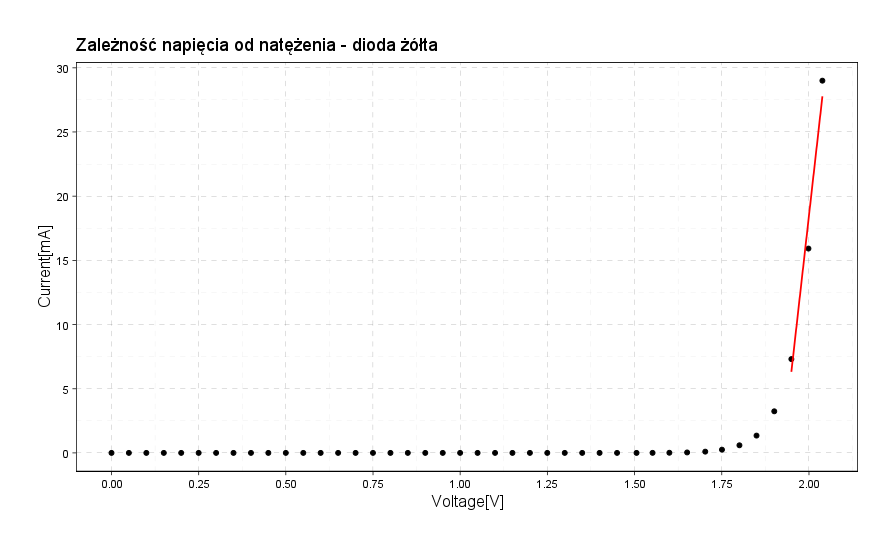
\includegraphics[scale = 0.41]{"F:/Projekty Intellij/Text/Fizyka3.1/44a/Img/Rplot01.png"}
    \end{center}
    \begin{center}
        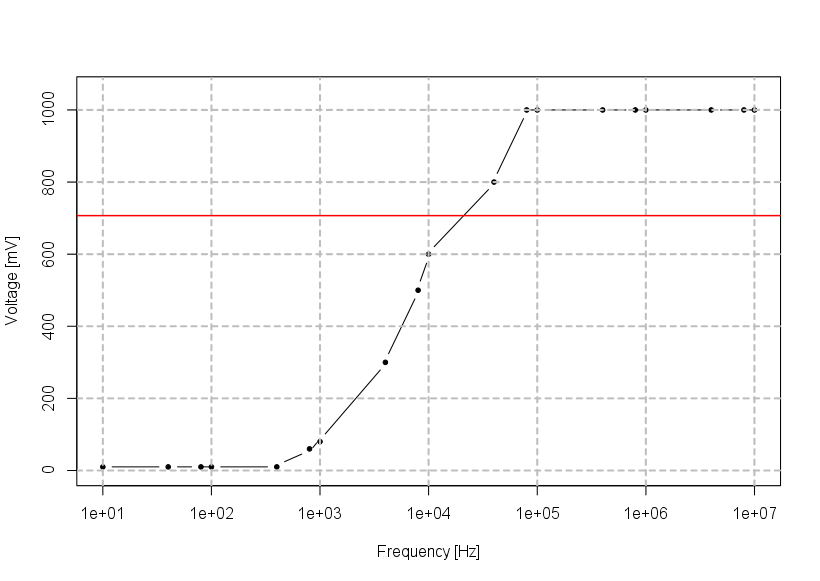
\includegraphics[scale = 0.41]{"F:/Projekty Intellij/Text/Fizyka3.1/44a/Img/Rplot02.png"}
    \end{center}
    \begin{center}
        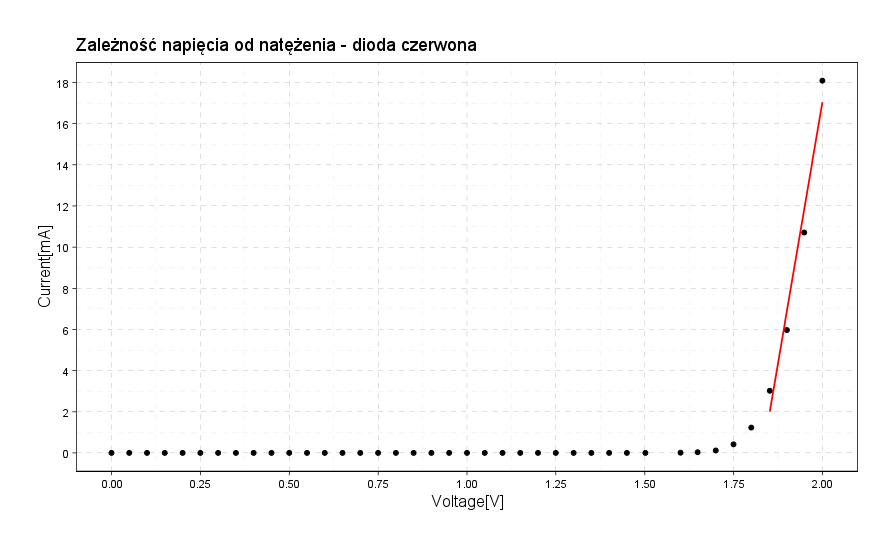
\includegraphics[scale = 0.41]{"F:/Projekty Intellij/Text/Fizyka3.1/44a/Img/Rplot03.png"}
    \end{center}
    \begin{center}
        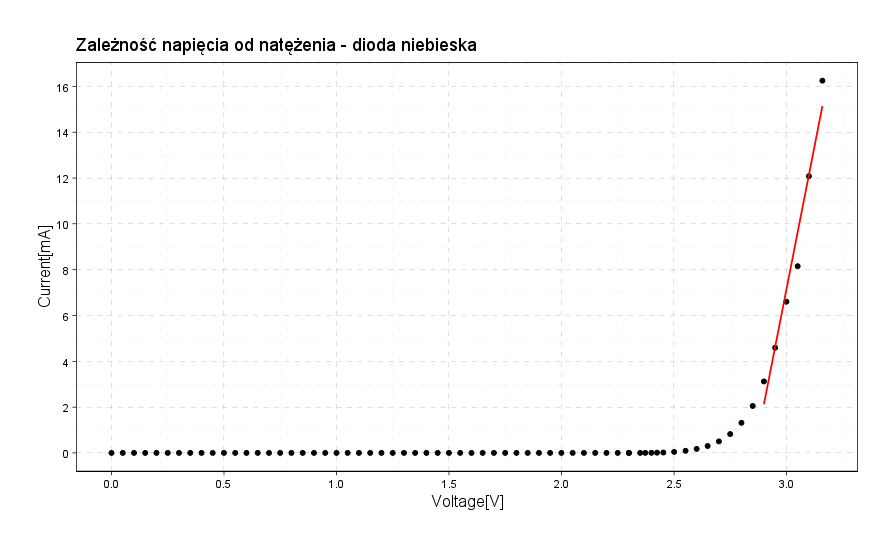
\includegraphics[scale = 0.41]{"F:/Projekty Intellij/Text/Fizyka3.1/44a/Img/Rplot04.png"}
    \end{center}

    \subsection*{Wykresy zależności rezystancji od temperatury i regresja liniowa próbki nr 4(Metal)}
    \begin{center}
        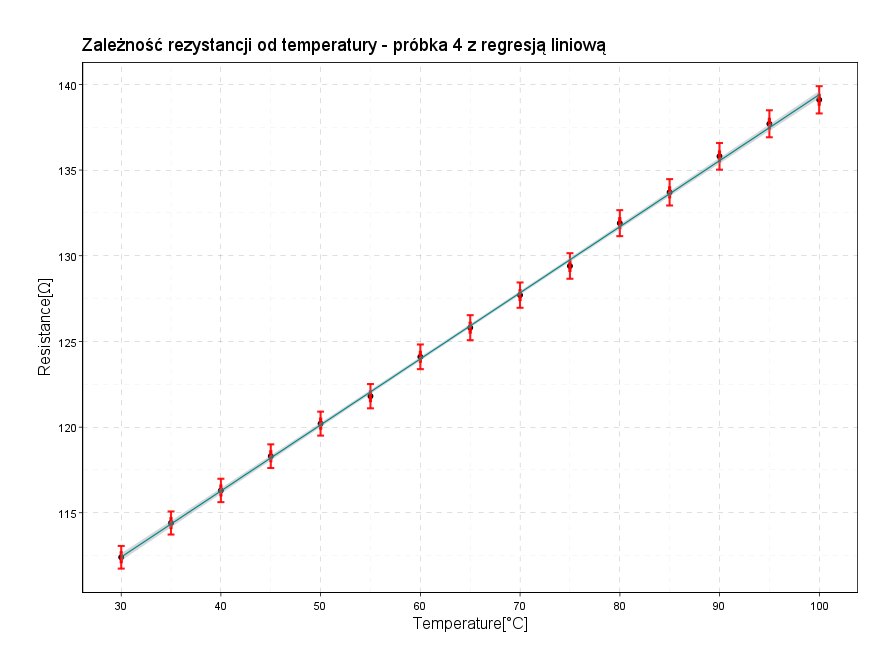
\includegraphics[scale = 0.45]{"F:/Projekty Intellij/Text/Fizyka3.1/44a/Img/Rplot05.png"}
    \end{center}
    Na podstawie regresji liniowej wyznaczono współczynniki a i b zależności oraz ich niepewności:
    \begin{gather*}
        a=0.3855[\frac{\Omega}{^\circ C}]\quad u(a)=0.0024[\frac{\Omega}{^\circ C}]\\
        b=100.85[\Omega]\quad\quad u(b)=0.16[\Omega]
    \end{gather*}
    Na podstawie powyższych danych wyliczono temperaturowy współczynnik oporu próbki nr 4 oraz niepewność tej wartości:
    \begin{gather*}
        \alpha=0.003823[\frac{1}{^\circ C}]\quad u_c(\alpha)=0.000025[\frac{1}{^\circ C}]
    \end{gather*}

    \subsection*{Wykresy zależności $ln(R_s)$ od $\frac{1000}{T}$ i regresja liniowa próbki\\ nr 2(Półprzewodnik)}
    \begin{center}
        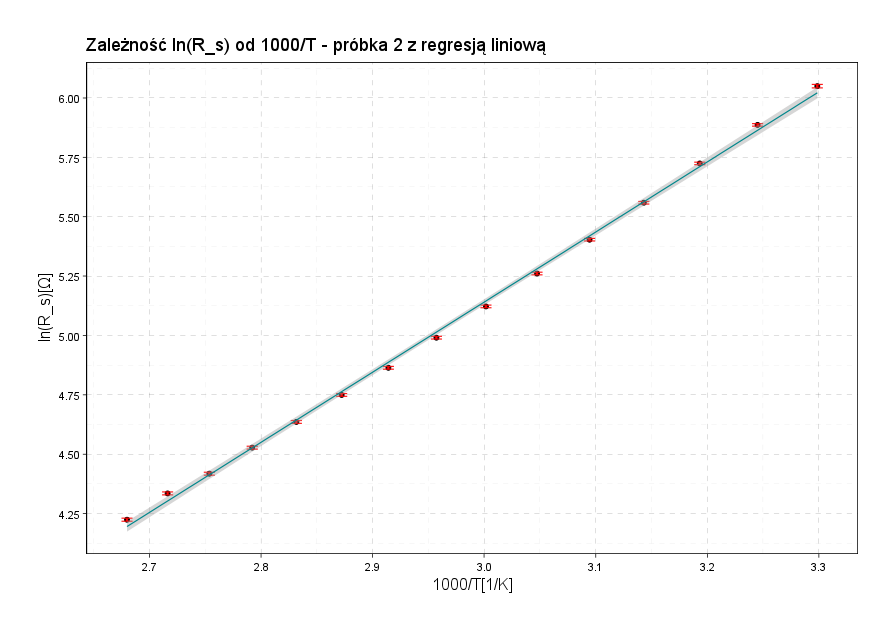
\includegraphics[scale = 0.45]{"F:/Projekty Intellij/Text/Fizyka3.1/44a/Img/Rplot06.png"}
    \end{center}
    Na podstawie regresji liniowej wyznaczono współczynniki A i B zależności oraz ich niepewności:
    \begin{gather*}
        A=2.952[\frac{\Omega}{^\circ C}]\quad u(A)=0.029[\frac{\Omega}{^\circ C}]\\
        B=-3.715[\Omega]\quad\quad u(B)=0.086[\Omega]
    \end{gather*}
    Na podstawie powyższych danych wyznaczono szerokość przerwy wzbronionej oraz jej niepewność:
    \begin{gather*}
        E_g=8.151\cdot 10^{-20}[J]=0.5087[eV]\\
        u_c(E_g)=0.079\cdot 10^{-20}[J]=0.0050[eV]
    \end{gather*}

    \newpage
    \section{Wnioski}
    Na podstawie doświadczenia udało się uzyskać wartości temperaturowego współczynnika oporu próbki nr 4 oraz
    szerokość przerwy wzbronionej dla próbki nr 2.\\
    Temperaturowy współczynnik oporu wyznaczony w ćwiczeniu wniósł:
    \begin{gather*}
        \alpha=0.003823\pm0.000025[\frac{1}{^\circ C}]
    \end{gather*}
    \indent Wartość ta w granicy błędu pomiarowego odpowiada dwóm pierwiastkom - srebru o współczynniku $0.003819[\frac{1}{^\circ C}]$
    oraz cynkowi o współczynniku $0.003847[\frac{1}{^\circ C}]$. W rzeczywistości materiał ten może być stopem metali który posiada
    tą specyficzną wartość temperaturowego współczynnika oporu.\\\\
    Przerwa energetyczna wyznaczona w doświadczeniu wyniosła:
    \begin{gather*}
        E_g=8.151\cdot 10^{-20}\pm 0.079\cdot 10^{-20}[J]\\
        E_g=0.5087\pm 0.0050[eV]
    \end{gather*}
    \indent Wartość ta odpowiada w granicy błędu Arsenkowi kadmu($Cd_{3As_2}$) którego przerwa energetyczna zawiera się w przedziale
    od 0.5[eV] do 0.6[eV].




\end{document}